\documentclass[11pt]{article}
\usepackage[top=1.00in, bottom=1.0in, left=1.1in, right=1.1in]{geometry}
\usepackage{Sweave}
\renewcommand{\baselinestretch}{1.1}
\usepackage{graphicx}
\usepackage{natbib}
\usepackage{amsmath}
\usepackage{rotating}
\usepackage{caption} 
\captionsetup[table]{skip=10pt}
\usepackage{hyperref}
\usepackage{xr-hyper}
\externaldocument{decsens}

\def\labelitemi{--}
\parindent=0pt

\begin{document}

\renewcommand{\refname}{\CHead{}}

\title{Supplementary information: A simple explanation for declining temperature sensitivity with warming} 

\author{E. M. Wolkovich  J. Auerbach, C. J. Chamberlain, D. M. Buonaiuto, \\ A. K. Ettinger, I. Morales-Castilla \& A. Gelman}
\date{} 
\maketitle  
\renewcommand{\thetable}{S\arabic{table}}
\renewcommand{\thefigure}{S\arabic{figure}}


\section{A first-hitting-time model of leafout}

Our model follows the general understanding of how warm temperatures (forcing) trigger leafout in temperate deciduous trees \citep{chuineJTB}. We use a first-hitting-time model, which describes the first time a random process hits a threshold, because of its broad applicability and conceptual simplicity. We define leafout day, $n_\beta$, as the day, $n$, that cumulative daily temperature, $S^n$, hits the threshold, $\beta$. \\ 

We derive the relationship between daily temperature and leafout in two common scenarios. In the first, we take the average daily temperature up until the leafout date. In the second, we take the average daily temperature over a fixed window, such as March 1st to April 30th. In both cases, we discretize time since, although many biological processes depend continuously on time, research typically measures time in discretized units, such as days, weeks, or months. % We assume the researcher knows the day temperatures start to accumulate, $n=0$. 

\subsection{Scenario 1: Using average daily temperature until the leafout date}

We use the following notation:
\begin{align*}
n & = \text{day since temperatures start to accumulate, }  n = 0, 1, ..., N\\
X_n & = \text{observed temperature on day $n$} \\
S_0^n & = \sum_{i = 0}^{n}X_i, \text{the cumulative daily temperature from day $0$ to day $n$}\\ 
M_0^n & = \frac{S_0^n}{n}, \text{the average daily temperature from day $0$ to day $n$}\\ 
\beta & = \text{the threshold of interest, } \beta > 0, \text{ (thermal sum required for leafout)}\\ % for example, F* or required GDD
n_{\beta} &  = \underset{n}{\text{argmin}} \ S_n > \beta, \text{the first day the cumulative daily temperature passes the threshold} \\
& \ \ \ \text{(for example, day of year (doy) of leafout).}
\end{align*} 

We model $X_n$ as a Gaussian random walk, $X_n \overset{\text{i.i.d}}{\sim} \text{normal}\left ( \alpha_0 + \alpha_1 n , \sigma \right )$, where $\alpha_0 > 0$ is the average temperature on day $n = 0$, $\alpha_1 > 0$ is the day-over-day increase in average temperatures, and $\sigma$ is the standard deviation. This model differs from the traditional Gaussian random walk because of the factor $n$.\\

This model has two important consequences: \\

(1) Leafout time is inversely related to average temperature at leafout time.\\

Under this model, $M_0^{n_{\beta}}$ and $n_{\beta}$ are inversely proportional. To see why, assume for the moment that the cumulative daily temperature hits the threshold exactly on leafout day. That is, $S_0^{n_\beta} = \beta$.
Then $$M_0^{n_{\beta}} = \frac{S_0^{n_{\beta}}}{{n_{\beta}}} = \frac{\beta}{{n_{\beta}}}$$ rearranging yields $${n_{\beta}} = \frac{\beta}{M_0^{n_{\beta}}}$$

Many global change biology studies use linear regression to quantify the relationship between $n_{\beta}$ and $M_0^{n_{\beta}}$ \citep[or similar metrics, see][for examples]{Wolkovich:2012n,piao2017,keenan2019}. Regressing $n_{\beta}$ on $M_0^{n_{\beta}}$ finds a best fit line to the inverse curve, ${n_{\beta}} = \frac{\beta}{M_0^{n_{\beta}}}$. The relationship is linearized with the logarithm transformation: $\log ({n_{\beta}}) = \log(\beta) - \log (M_0^{n_{\beta}})$. That is, $\log(n_{\beta})$ is linear in log-average daily temperature with slope -1 and intercept $\log(\beta)$. \\ % (e.g., in simulations in Fig. \ref{fig:basicsimswpep} is -1, and intercept is $\log(200)=5.3$)

(2) The variance of the average temperature may decreases as temperatures rise.\\

Under the model, the mean and variance of $M_0^n$ are E$(M_0^n | \alpha_0, \alpha_1) = \frac{1}{n} \sum_{i=0}^n ( \alpha_0 + \alpha_1 i )  = \alpha_0 + \alpha_1 \frac{(n + 1)}{2} $ and Var$(M_0^n | \alpha_0, \alpha_1) = \frac{\sigma^2}{n}$.\\

By the law of total variance,

\begin{align*}
\text{Var}(M_0^n)& = \text{E}(\text{Var}(M_0^n | \alpha_0, \alpha_1)) + \text{Var}(\text{E}(M_0^n | \alpha_0, \alpha_1))\\
& = \frac{\sigma^2}{n} + \text{Var}(\alpha_0 + \alpha_1 \frac{n+1}{2})\\
& = \frac{\sigma^2}{n} + \text{Var}(\alpha_0) + \frac{(n+1)^2}{4} \text{Var}(\alpha_1) + (n+1) \text{Cov}(\alpha_0, \alpha_1)
\end{align*}

As temperatures rise and leafout date becomes earlier, the variance of the average temperature will decline---provided the variation in temperatures, $\sigma$, is sufficiently small. 

\subsection{Scenario 2: Using average daily temperature over a fixed window}
% See email from J Auerbach on 13 Apr 2020 ... The distribution of the average temperature over the window, and the distribution of leafout given the average temperature over a window

We slightly modify the notation:
\begin{align*}
n & = \text{day since temperatures start to accumulate, }  n = 0, \ldots, a, \ldots, b\\
X_n & = \text{observed temperature on day $n$} \\
S_a^n & = \sum_{i = a}^{n}X_i, \text{the cumulative daily temperature from day $a$ to day $n$}\\ 
M_a^n & = \frac{S_a^n}{n-a}, \text{the average daily temperature from day $a$ to day $n$}\\ 
\beta & = \text{the threshold of interest, } \beta > 0, \text{ (thermal sum required for leafout)}\\
n_{\beta} &  = \underset{n}{\text{argmin}} \ S_0^n > \beta, \text{the first day the cumulative daily temperature passes the threshold} \\
& \ \ \ \text{(for example, day of year (doy) of leafout).}
\end{align*} 

As before, we model $X_n$ as a Gaussian random walk, $X_n \overset{\text{i.i.d}}{\sim} \text{normal}\left ( \alpha_0 + \alpha_1 n , \sigma \right )$, where $\alpha_0 > 0$ is the average temperature on day $n = 0$, $\alpha_1 > 0$ is the day-over-day increase in average temperatures, and $\sigma$ is the standard deviation. We make the additional assumption that $X_n \geq 0$ for all $n$ and $a < n_{\beta} < b$. That is, the cumulative temperature acquired by the plant always increases. \\ % Note: This is an important assumption ... I started to add text about this, but decided to skip it. We could, and probably best to reference \citep{gusewell2017} if do.

Note that \\

$S_a^b \sim \text{normal}\left ( \alpha_0 (b - a) + \frac{\alpha_1}{2} (b-a)(b+a+1), \sigma \sqrt{b - a} \right )$ \\

$M_a^b \sim \text{normal}\left ( \alpha_0 + \frac{\alpha_1}{2} (b+a+1), \frac{\sigma}{\sqrt{b - a}} \right )$ \\ % average daily temp

$S_n^b - S_a^b  \sim \text{normal}\left ( \alpha_0 (b - a - n) + \frac{\alpha_1}{2} ( (b-n)(b+n+1) - a(a+1) ), \sigma \sqrt{b + a - n} \right )$ \\ % sum of n to b (post leafout sum) - sum full window

so that
\begin{align*}
Pr \left ( n_{\beta} \leq n \ \big |  \ M_{a}^b = m \right ) &= Pr \left ( n_{\beta} \leq n \ \big |  \ S_a^b = (b-a) m \right ) \\ % m is the (observed) average temperature in the time window a,b
&= Pr \left ( S_0^n \geq \beta \ \big |  \ S_a^b = (b-a) m \right ) \\
&= Pr \left ( S_n^b \leq (b-a) m + S_0^a - \beta \right ) \\
&= Pr \left ( S_n^b - S_0^a \leq (b-a) m - \beta \right ) \\
&= \Phi \left ( \frac{(b-a) m - \beta -    [ \alpha_0 (b - a - n) + \frac{\alpha_1}{2} ( (b-n)(b+n+1) - a(a+1) ) ] }{\sigma \sqrt{b + a - n}} \right )
\end{align*}
\vspace{3ex}

The distribution of $M_a^b$ shows that consequence (2) above still holds with this model. Consequence (1) no longer holds directly, but will in many situations where average daily temperature until an event correlates strongly with average daily temperature because the window is chosen based, in part, on the expected hitting time (Figs. \ref{fig:simslog}-\ref{fig:basicsims}). We note two additional consequences: \\

(3) The conditional median is quadratic in $n$: \\

\begin{align*}
\frac{1}{2} & \overset{\text{set}}{=} Pr \left ( n_{\beta} \leq n \ \big |  \ M_a^b = m \right )  \\
& \Rightarrow 0 = (b-a) m - \beta -    [ \alpha_0 (b - a - n) + \frac{\alpha_1}{2} ( (b-n)(b+n+1) - a(a+1) ) ] \\
& \Rightarrow m = \frac{1}{(a-b)} [-  \beta -  \alpha_0 (b - a - n) - \frac{\alpha_1}{2} ( (b-n)(b+n+1) - a(a+1) ) ] \\
& \phantom{\Rightarrow m} \ = \frac{1}{(a-b)} [- \beta -  \alpha_0 (b - a ) - \frac{\alpha_1}{2} (b-a)(b+a+1) ] + \frac{\alpha_0 + \frac{\alpha_1}{2}}{(a-b)} n +  \frac{ \frac{\alpha_1}{2} }{(a-b)} n^2  \\
& \phantom{\Rightarrow m} \ := \gamma_0 + \gamma_1 n + \gamma_2 n^2 
\end{align*}

(4) The conditional mean and variance are sums of negative sigmoids, according to the following identities \\

$E \left ( n_{\beta} \ \big |  \ M_{a}^b = m \right ) =  \sum_{n=0}^{\infty} Pr \left ( n_{\beta} \geq n \ \big |  \ M_{a}^b = m \right )$ \\

$E \left ( n_{\beta}^2 \ \big |  \ M_{a}^b = m \right ) =  \sum_{n=0}^{\infty} \ n \  Pr \left ( n_{\beta} \geq n \ \big |  \ M_{a}^b = m \right )$ \\

\section{Results using long-term empirical data from PEP725} %http://www.pep725.eu}
To examine how estimated sensitivities shift over time, we selected sites of two common European tree species (silver birch, \emph{Betula pendula}, and European beech, \emph{Fagus sylvatica}) that have long-term observational data of leafout, through the Pan European Phenology Project \citep[PEP725,][]{Templ2018}. We used a European-wide gridded climate dataset \emph{\citep[{\normalfont E-OBS},][]{cornes2018}} to extract daily minimum and maximum temperature for the grid cells where observations of leafout for these two species were available. We used sites with complete leafout data across both our 10-year (and 20-year) windows to avoid possible confounding effects of shifting sites over time (see Tables \ref{tab:pep10yr}-\ref{tab:pep20yr} for numbers of sites per species x window). \\

Our estimates of temperature sensitivity from a linear model using untransformed variables show a decline in sensitivity with recent warming for \emph{Betula pendula} over 10 and 20-year windows, but no decline for \emph{Fagus sylvatica}; using logged variables estimates appeared more similar over time or sometimes suggested an increase in sensitivity (see Figs. \ref{fig:pepper10yr}-\ref{fig:pepper20yr}, Tables \ref{tab:pep10yr}-\ref{tab:pep20yr}). This shift in estimated sensitivity when regressing with untransformed versus logged variables suggests the declining estimates with untransformed variables may not be caused by changes in the underlying mechanisms of leafout (i.e., reduced winter chilling) and driven instead by using linear regression for a non-linear process. This hypothesis is supported further by large declines in variance of leafout in recent decades. \\

Shifts in variance provide another hurdle to robust estimates of temperature sensitivity. Previous work has highlighted how shifting temperature variance (over space and/or time) could lead to shifting estimates of temperature sensitivities \citep{keenan2019}, but our results stress that variance in both leafout and temperature are shifting. If both shift in step, estimates would not be impacted by changes in temperature variance, but our results suggest variance in temperature---for these data---has declined more than variance in leafout, though both have declined substantially in recent decades (Tables \ref{tab:pep10yr}-\ref{tab:pep20yr}). \\

Estimated sensitivities for the empirical data (PEP725) using logged variables are far lower than the value obtained in our simulations (-1). This likely results from a contrast between our simulations---where we can accurately define the temperature plants experience and the temporal window that drives leafout---and our empirical data, where we do not know how measured temperatures translate into the temperatures that plants accumulate and where we have no clear method to define the relevant temporal window \citep{gusewell2017}. \\

These results highlight how the acceleration of biological time due to climate change requires researchers to clarify their assumptions. Expecting temperature sensitivity to remain constant as temperatures rise assumes the relationship between response and temperature is proportional. But the underlying biological processes suggest this relationship is seldom proportional, or even linear. In fact, when our model holds, declining sensitivity with rising temperatures should be the null hypothesis of any analysis of temperature sensitivity based on linear regression or similar methods. \\ % Traditional methods that reliably infer mechanisms at historic temperatures may no longer be applicable at higher temperatures.

\emph{References}
\vspace{-6ex}
\bibliographystyle{..//refs/bibstyles/amnat.bst}
\bibliography{..//refs/decsens.bib}
 
\clearpage
\section{Tables}
\vspace{-3ex}
% latex table generated in R 3.5.1 by xtable 1.8-3 package
% Sun Jul  5 13:38:16 2020
\begin{table}[ht]
\centering
\caption{Climate and phenology statistics for two species (\emph{Betula pendula, Fagus sylvatica}, across 45 and 47 sites respectively) from the PEP725 data across all sites with continuous data from 1950-1960 and 2000-2010. ST is spring temperature from 1 March to 30 April, ST.leafout is temperature 30 days before leafout, and GDD is growing degree days 30 days before leafout. Slope represents the estimated sensitivity using untransformed leafout and ST, while log-slope represents the estimated sensitivity using log(leafout) and log(ST). We calculated all metrics for for each species  x site x 10 year period before taking mean or variance estimates. See also Fig. \ref{fig:pepper10yr}.} 
\label{tab:pep10yr}
\begingroup\footnotesize
\begin{tabular}{|p{0.1\textwidth}|p{0.15\textwidth}|p{0.09\textwidth}|p{0.1\textwidth}|p{0.07\textwidth}|p{0.07\textwidth}|p{0.07\textwidth}|p{0.07\textwidth}|p{0.07\textwidth}|}
  \hline
years & species & mean (ST) & mean (ST.leafout) & var (ST) & var (leafout) & mean (GDD) & slope & log-slope \\ 
  \hline
1950-1960 & \emph{Betula pendula} & 5.6 & 7.0 & 3.4 & 110.5 & 71.7 & -4.3 & -0.17 \\ 
  2000-2010 & \emph{Betula pendula} & 6.6 & 6.8 & 1.2 & 47.0 & 64.6 & -3.6 & -0.22 \\ 
  1950-1960 & \emph{Fagus sylvatica} & 5.6 & 7.5 & 3.3 & 71.9 & 83.8 & -2.8 & -0.11 \\ 
  2000-2010 & \emph{Fagus sylvatica} & 6.7 & 7.7 & 1.2 & 38.3 & 86.7 & -3.4 & -0.20 \\ 
   \hline
\end{tabular}
\endgroup
\end{table}

% latex table generated in R 3.5.1 by xtable 1.8-3 package
% Sun Jul  5 13:38:16 2020
\begin{table}[ht]
\centering
\caption{Climate and phenology statistics for two species (\emph{Betula pendula, Fagus sylvatica}, across 17 and 24 sites respectively) from the PEP725 data across all sites with continuous data from 1950-2010. ST is spring temperature from 1 March to 30 April, ST.leafout is temperature 30 days before leafout, and GDD is growing degree days 30 days before leafout. Slope represents the estimated sensitivity using untransformed leafout and ST, while log-slope represents the estimated sensitivity using log(leafout) and log(ST). We calculated all metrics for for each species  x site x 20 year period before taking mean or variance estimates. See also Fig. \ref{fig:pepper20yr}.} 
\label{tab:pep20yr}
\begingroup\footnotesize
\begin{tabular}{|p{0.1\textwidth}|p{0.15\textwidth}|p{0.09\textwidth}|p{0.1\textwidth}|p{0.07\textwidth}|p{0.07\textwidth}|p{0.07\textwidth}|p{0.07\textwidth}|p{0.07\textwidth}|}
  \hline
years & species & mean (ST) & mean (ST.leafout) & var (ST) & var (leafout) & mean (GDD) & slope & log-slope \\ 
  \hline
1950-1970 & \emph{Betula pendula} & 5.8 & 7.1 & 2.6 & 79.9 & 72.5 & -4.3 & -0.19 \\ 
  1970-1990 & \emph{Betula pendula} & 5.9 & 7.2 & 1.3 & 104.8 & 72.2 & -6.1 & -0.33 \\ 
  1990-2010 & \emph{Betula pendula} & 6.8 & 6.7 & 0.9 & 36.2 & 60.0 & -3.3 & -0.21 \\ 
  1950-1970 & \emph{Fagus sylvatica} & 5.6 & 7.6 & 2.7 & 63.4 & 86.0 & -3.1 & -0.12 \\ 
  1970-1990 & \emph{Fagus sylvatica} & 5.6 & 7.5 & 1.3 & 56.2 & 81.3 & -2.5 & -0.16 \\ 
  1990-2010 & \emph{Fagus sylvatica} & 6.7 & 7.3 & 1.2 & 31.4 & 76.0 & -3.4 & -0.19 \\ 
   \hline
\end{tabular}
\endgroup
\end{table}

\clearpage
\section{Figures}


\begin{figure}[h!]
\centering
\noindent 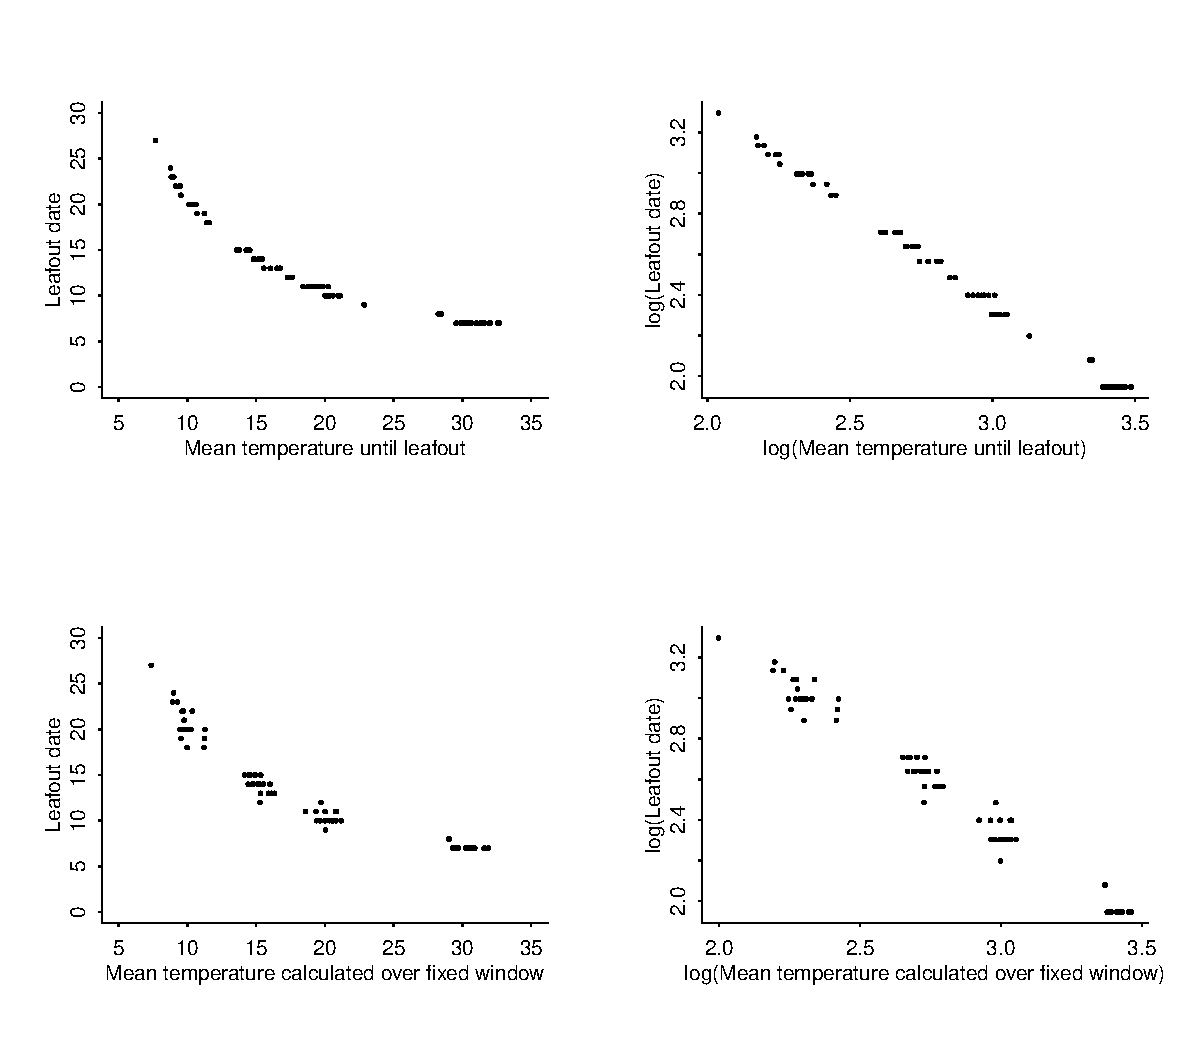
\includegraphics[width=1\textwidth]{..//analyses/figures/simslogging.pdf}
\caption{\textbf{Simulated leafout as a function of temperature across different temperatures highlights non-linearity of process.} Here we simulated sets of data where leafout constantly occurs at 200 growing degree days (thermal sum of mean daily temperatures with 0$^{\circ}$C as base temperature) across mean temperatures of 10, 15, 20 and 30$^{\circ}$C (constant SD of 4), we calculated estimated mean temperature until leafout date (top row) or across a fixed window (bottom row, similar to estimates of `spring temperature'). While within any small temperature range the relationship may appear linear, its non-linear relationship becomes clear across the greater range shown here (left). Taking the log of both leafout and temperature (right) linearizes the relationship.}
\label{fig:simslog} % % decsensSims.R
\end{figure}

\clearpage
\begin{figure}[h!]
\centering
\noindent 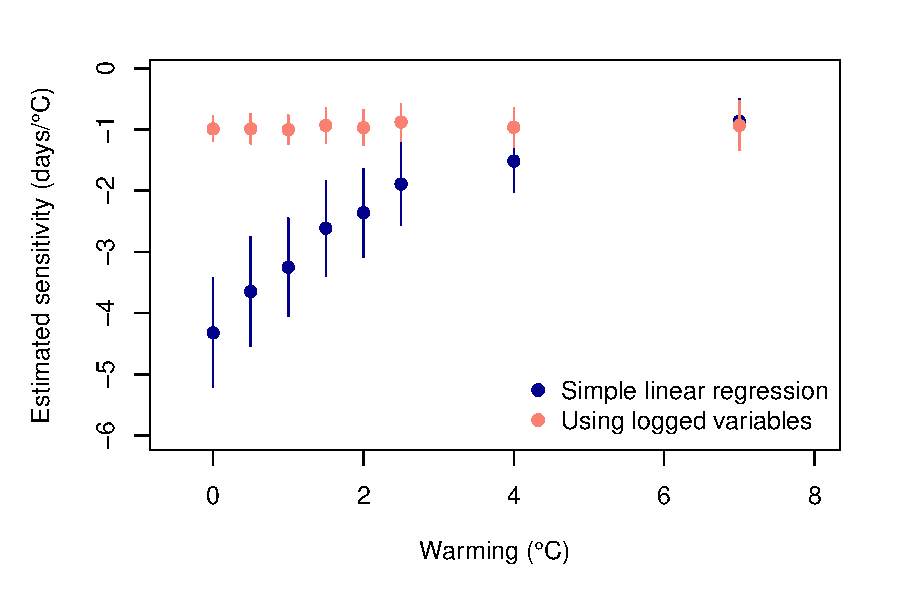
\includegraphics[width=0.75\textwidth]{..//analyses/figures/basicsims.pdf}
\caption{\textbf{A simple model generates declining sensitivities with warming.} We show declines in estimated sensitivities with warming from simulations (top: using average temperature until leafout, bottom: using a fixed window) with no underlying change in the biological process when sensitivities were estimated with simple linear regression (``Simple linear regression''). This decline disappears using regression on logged predictor and response variables (``Using logged variables'').}
\label{fig:basicsims} % decsensSims.R
\end{figure}

\begin{figure}[h!]
\centering
\noindent 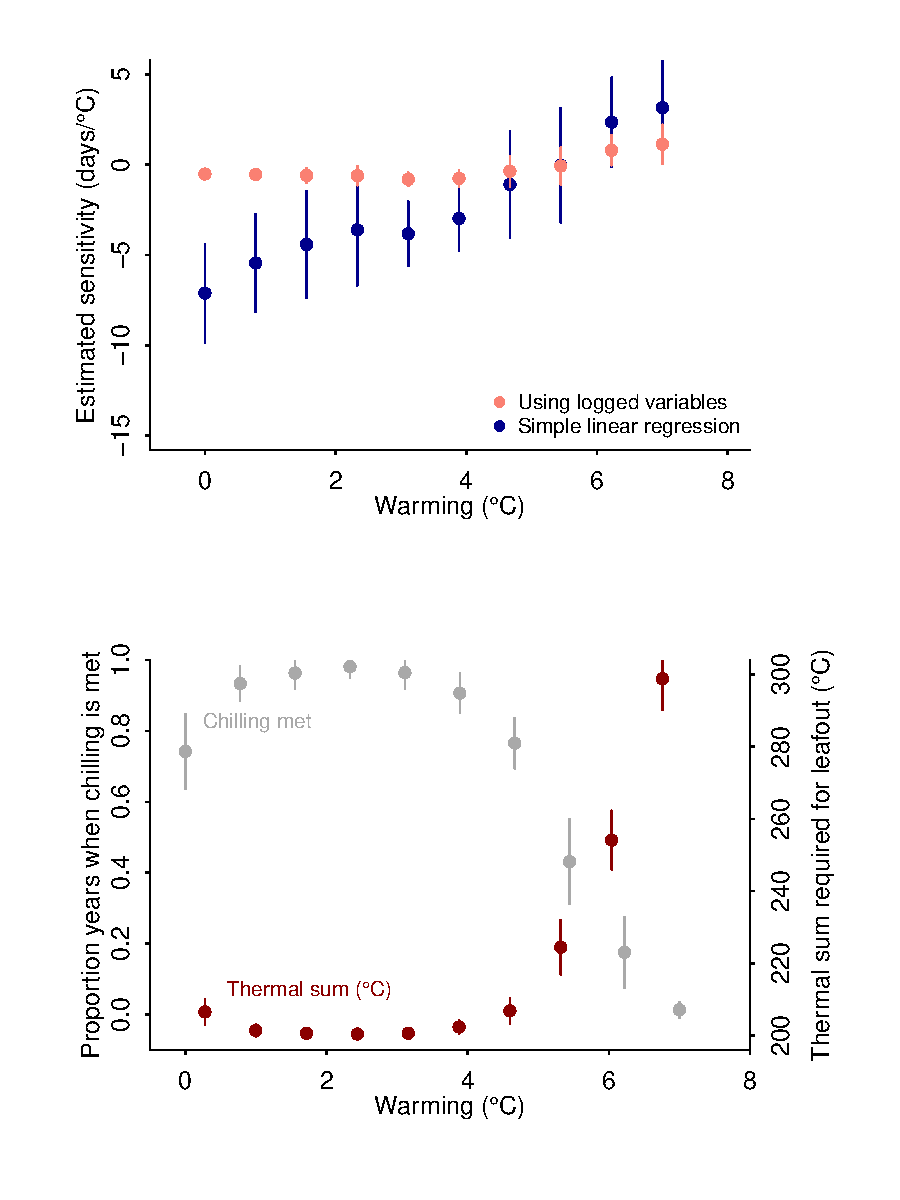
\includegraphics[width=0.8\textwidth]{..//analyses/figures/shiftingcuessims_2panels.pdf}
\caption{\textbf{Simulated leafout as a function of temperature across different levels of warming with shifts in underlying biology.} Here we simulated sets of data where leafout occurs at a thermal sum of 200 (sum of mean daily temperatures with 0$^{\circ}$C as base temperature) when chilling is met, and requires a higher thermal sum when chilling is not met. We show estimated sensitivities in the top panel, and the shifting cues in the bottom panel. } % Note that this model is non-identifiable as the same response data could come from a forcing-only model or a chilling and forcing model. 
\label{fig:simsshiftcues} % decsensMo.R
\end{figure}

\clearpage
\begin{figure}[h!]
\centering
\noindent 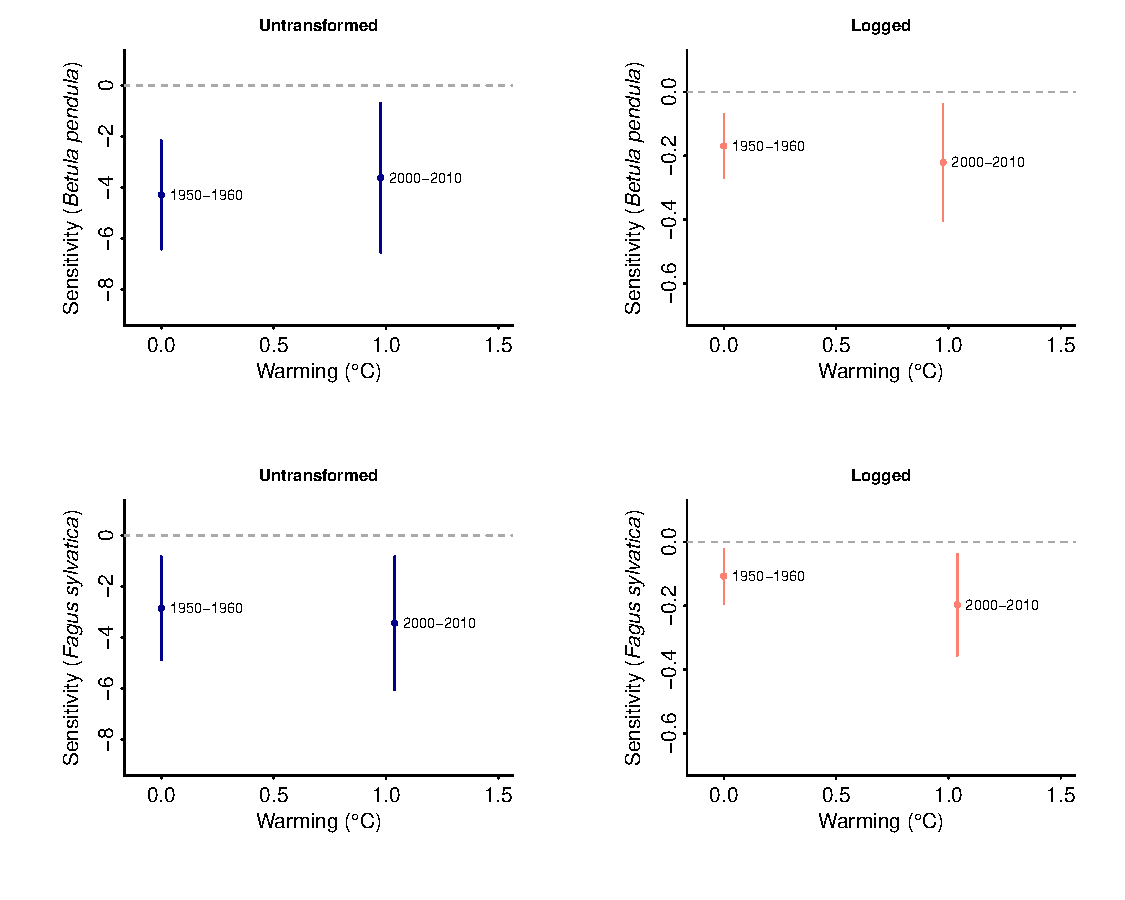
\includegraphics[width=1\textwidth]{..//analyses/figures/basicpep195020102spp4paneladj.pdf}
\caption{\textbf{Sensitivities from PEP725 data using 10 year windows of data} for two species (top -- \emph{Betula pendula}, bottom -- \emph{Fagus sylvatica}; all lines show 78\% confidence intervals from linear regressions). Amounts of warming are calculated relative to 1950-1960 and we used only sites with leafout data in all years shown here. See Table \ref{tab:pep10yr} for further details. }
\label{fig:pepper10yr} % pepplotting.R
\end{figure}

\clearpage
\begin{figure}[h!]
\centering
\noindent 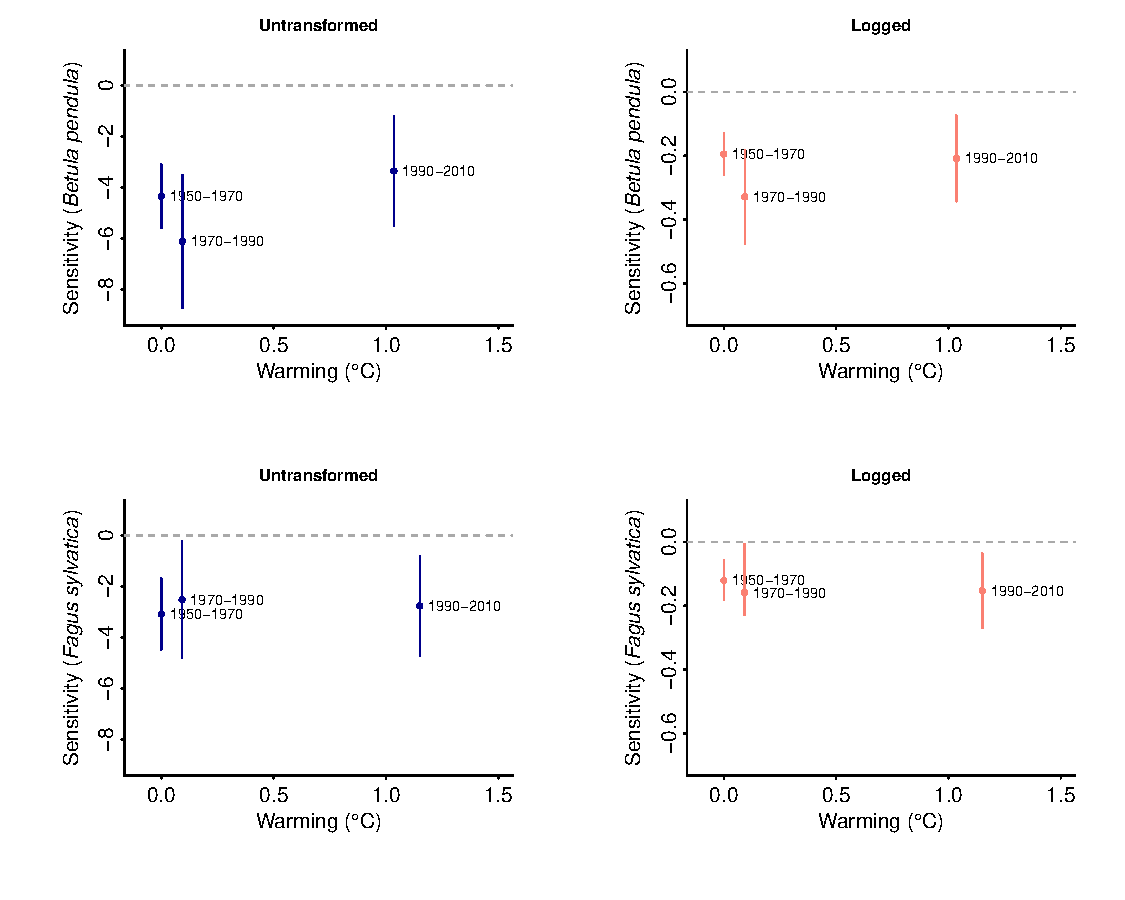
\includegraphics[width=1\textwidth]{..//analyses/figures/basicpep1950to20002spp4paneladj.pdf}
\caption{\textbf{Sensitivities from PEP725 data using 20 year windows of data} for two species (top -- \emph{Betula pendula}, bottom -- \emph{Fagus sylvatica}; all lines show 78\% confidence intervals from linear regressions). Amounts of warming are calculated relative to 1950-1970 and we used only sites with leafout data in all years shown here. See Table \ref{tab:pep20yr} for further details. }
\label{fig:pepper20yr} % pepplotting.R
\end{figure}


\end{document}







